\section{Teilbericht Fahrzeuge}

Ziel der Teilgruppe Fahrzeuge ist es, einen autonomen Transport zwischen den Rampen zu realisieren. Dafür sollen die Volksbots in der Lage sein, auf die eingehenden Aufträge zu reagieren.
Dies beinhaltet die Teilnahme an Auktionen ( Jobverteilung ), welche durch eine Aufwandsabschätzung des Auftrages eines jeden Volksbots entschieden werden. Nach der Zuweisung an den besten geeigneten Volksbot soll dieser das Paket von der entsprechenden Startrampe holen und zur Zielrampe transportieren.

Folgendes wird in den nächsten Unterkapiteln behandelt:

\begin{itemize}
	\item Anforderungskatalog an das Endsystem
	\item Beschreibung der Komponenten
	\item Werkzeuge
	\item Architektur
	\item Implementierung
	\item Erreichte Funktionalitäten
	\item Herausforderungen
	\item Ausblick
\end{itemize} 

\subsection{Anforderungen}

\begin{itemize}

\item \textbf{Aufträge}: Aufträge enthalten den Start- und Zielpunkt, welche in der Umgebungskarte gesetzt werden. Diese werden für weitere Berechnungen verwendet.

\item \textbf{Bieten}: Ein Volksbot ist in der Lage an einer Auftragsverteilung teilzunehmen, sofern er noch keinen Auftrag ausführt und sein Energievorrat nicht das kritische Minimum erreicht hat. Die Teilnahme beinhaltet eine Aufwandsschätzung anhand einer Distanzfunktion, sowie dem aktuellen Energiezustand. 

\item \textbf{Planung}: Bei der Erteilung eines Auftrages und dem Bieten für einen Auftrag, muss der Volksbot die Route vom aktuellen Standort zum Startpunkt berechnen. Dies gilt ebenso vom Startpunkt zum Endpunkt.

\item \textbf{Navigation}: Für die Routenplanung soll der kürzeste Weg verwendet werden, sofern möglich die direkte Verbindung zum gewüschten Ziel. Die Planung, Navigation und Positionierung erfolgt dabei auf dem entsprechenden Notebook.

\item \textbf{Positionierung}: Die Umgebungskarte ist jedem Volksbot bekannt. Bei Bewegungen aktualisiert dieser seine Position mittels Odometrie, um die geplante Route korrekt zu befahren. Zur lokalen Unterstützung werden die Laserscanner verwendet werden. Startpunkt eines Volksbots wird statisch definiert.

\item \textbf{Synchronisation}: Jegliche Information eines Volksbots wird an die Simulation übermittelt. Dies beinhaltet neben der aktuellen Position auch den Ladezustand, sowie den Energievorrat eines Volksbots.

\item \textbf{Feinsteuerung}: Das genaue Heranfahren an ein Objekt, sei es die Ladestation oder eine Rampe, erfolgt mit Hilfe der Laserscanner. 

\item \textbf{Überabe}: Bei Einnahme der korrekten Position zum Be- oder Entladen des Volksbots findet ein Datenaustausch mit der entsprechenden Rampe statt. Es folgt eine kooperative Interaktion beider, bis der Volksbot das Paket erhalten oder abgeladen hat.

\item \textbf{Energiemanagement}: Sobald ein Volksbot seinen kritischen Energiezustand erreicht, werden alle Auftragsverteilungen ignoriert und der Bot setzt die Dockingstation als primäres Ziel. Sollten mehrere Bots die Ladestation ansteuern, oder diese bereits belegt sein, so wird der Folgeablauf durch eine Queue oder ein anderes Verfahren geregelt.

\item \textbf{Kollisionsvermeidung}: Sobald eine Kollision mit einem festen oder mobilen Objekt erkannt wird, wird eine Neuberechnung, Umplanung oder ein Ausweichverfahren eingeleitet um entsprechend zu reagieren.

\end{itemize}



\subsection{Beschreibung der Komponenten}

Bei dem Volksbot handelt es sich um einen modular aufgebauten und mobilen Roboter, der vom Frauenhofer-Institut IAIS entwickelt wurde. Die in diesem Projekt verwendeten Prototypen bestehen aus drei zentralen Elementen. 

	\begin{figure}[h!]
		\centering
			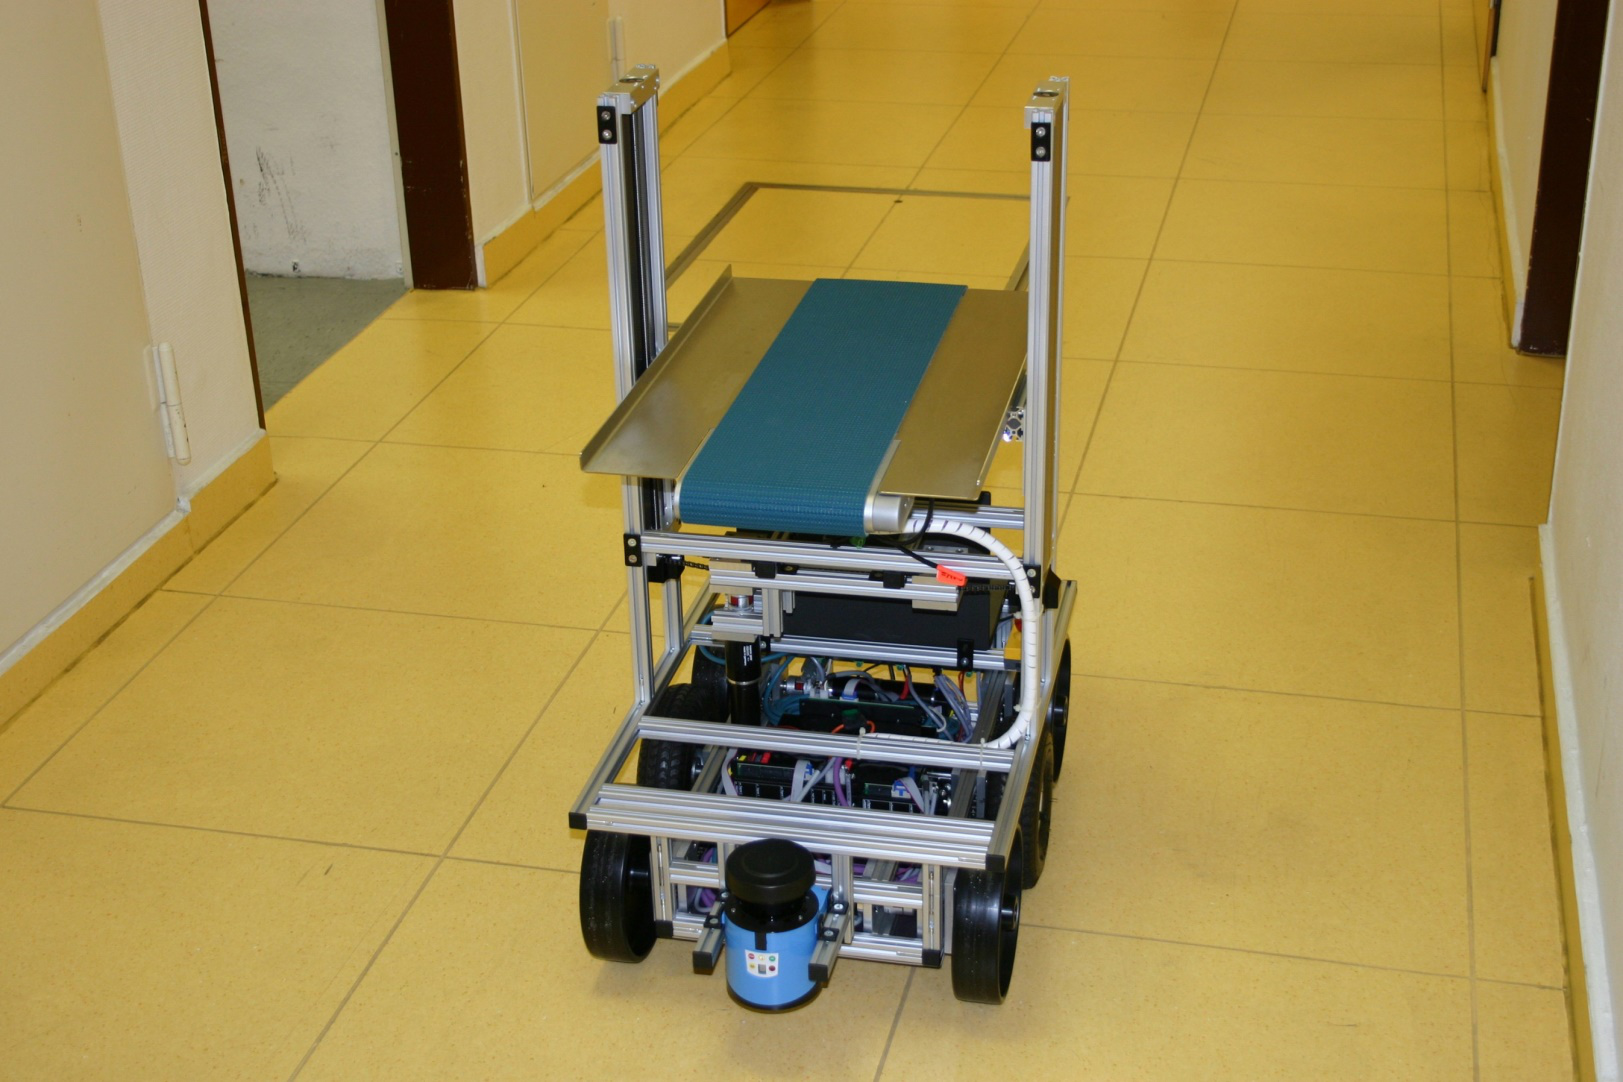
\includegraphics[width=0.9\textwidth]{Volksbot.png}
			\caption{Darsellung eines Volksbots}
			\label{Volksbot}
	\end{figure}	

\begin{itemize}

\item \textbf{Fahreinheit}
Die Fahreinheit wird aus zwei Maxonantrieben links und rechts, sowie dem Gerüst des Bots gebildet. Vorne befindet sich ein SICK LMS100 Laserscanner,  hinten ein SICK TiM310 Laserscanner. Angesteuert werden die Hardwarekomponenten mit Hilfe von vier Epos2 Controllern, die mit Hilfe einer CAN-Verbindung ansteuerbar sind. 

\item \textbf{Hub-Förderband}
Zum Transportieren der Pakete ist der Volksbot mit einer Hubeinheit ausgestattet, die zum Schutz vor Überdrehungen zwei Hallsensor auf beiden seiten beinhaltet. Des weiteren befindet sich auf der Hubeinheit ein Förderband, an dem sich zwei Lichtschranken befinden. Diese sollen zur Ermittlung des Beladungszustandes dienen. 

\item \textbf{Steuereinheit}
Gesteuert wird das System mit Hilfe eines Notebooks, welches unter Ubuntu mit Hilfe des Robot Operating System (ROS) die Hardware anspricht. Auf dem Notebook werden ausserdem sämtliche 
Berechnungen durchgeführt. Neben der Ansteuerung der EPOS2 Controller wird der SICK LMS100 über eine Ethernet Schnittstelle angeschlossen. Zur Kommunikation mit den Rampen wird zusätzlich ein MICAZ Modul verwendet, welches mittels einer USB Schnittstelle mit dem Notebook verbunden ist.

\end{itemize}
\subsection{Werkzeuge}
Beschreibung ROS. 
Wichtige Funktionen in ROS:
\begin{itemize}
\item Publish
\item Subscribe
\item ...
\end{itemize}
\subsubsection{Robot Operating System (ROS)}

\subsubsection{Was ist ROS}
Es gibt viele Robotik-Frameworks, die spezifisch für präzise Anwendungen, für Prototypen,
erstellt wurden. ROS strebt da eher das Allgemeine an. Das »Robot Operating System«
(ROS) ist ein Open-Source Framework für individuelle Roboter, das sich in der
Robotikforschung in den letzten Jahren etabliert hat und ein großes Repertoire an Software-Komponenten und -Werkzeugen für Robotikapplikationen bietet.\\
Die Entwicklung begann 2007 am Stanford Artificial Intelligence Laboratory im Rahmen des
Stanford-AI-Robot-Projektes (STAIR). Heute wird es hauptsächlich am Robotik Institut Willow
Garage weiterentwickelt. Seit April 2012 wird ROS von der neu gegründeten,
gemeinnützigen Organisation Open Source Robotics Foundation (OSRF) unterstützt. Die
Bibliotheken von ROS setzen auf Betriebssysteme wie Linux, Mac OS X oder Windows auf.
ROS ist nicht von einer spezifischen Sprache abhängig. Heutzutage gibt es 3 Grundlibraries
für ROS, die jeweils auf Python, Lisp und C++ ausgerichtet sind. Zwei Exmperimentier-
Librairies sind für Java und Lua erhältlich.
\subsubsection{Was will ROS?}
\begin{itemize}
 \item ROS will unterstützen, Code für Forschung und Entwicklung wiederzuverwenden
 \item loser Verbund von individuellen Programmteilen (Nodes)
 \item einzelne Programmteile können einfach geteilt und verbreitet werden (Packages und Stacks)
 \item ROS stellt Repositories zu Verfügung, um dort Code zu teilen \cite{ROS:2014:Online}
(http://www.ros.org/browse)
\end{itemize}
\subsubsection{Was kann ROS?}
Die Hauptbestandteile und Hauptaufgaben von ROS sind Hardwareabstraktion; Gerätetreiber; Implementierung 
von viel genutzten Funktionalitäten; Inter-Prozess-Kommunikation; Paket-Management
\subsubsection{Aufgaben des ROS}
\begin{itemize}
 \item Interprozesskommunikation (IPC)
 \begin{itemize}
\item Problematik der Kommunikation zwischen verschiedenen Systemen des Roboters
\item Sicherheitseinstellung bei der Übertragung
\item Anforderung an die Geschwindigkeit / Schnelligkeit der Kommunikation
\item Koordination von Nachrichten durch zentralen Master
\end{itemize}
\item Paketverwaltung – Packages
\begin{itemize}
 \item ROS ist durch Softwarepakete (sogn. Packages) aufgebaut
 \item Ein Package beinhaltet Laufzeitprozesse (Nodes); ROS abhängige Bibliotheken;
Datensätze; Konfigurationsdateien;3rd Party Software
 \item Packages sind dazu, da um Code wiederverwendbar zu machen
\end{itemize}
\item Paketverwaltung – Stacks
\begin{itemize}
\item Sammlung von Paketen (Packages)
\item Der Sinn ist, dass Stacks die Verteilung und Verwendbarkeit von Code
vereinfachen
\item Meist viele Packages ähnlicher Aufgaben in einem Stack verpackt
\end{itemize}
\item Message (msg)
\begin{itemize}
 \item  Messages werden verwendet um unter ROS Nachrichten zwischen Knoten und
Topics auszutuaschen
\item Dafür verwendet ROS eine einfache Beschreibung der Datentypen in Textdateien
\item Durch diese Beschreibung kann für unterschiedliche Sprachen Code autogeneriert
werden
\item Diese sind in .msg-Dateien im msg- Unterverzeichnis eines ROS-Pakets abgelegt
\item Eigene Message-Typen sind mit Paket Ressource-Namen bezeichnet
\item Standard Messages sind mit std\_msg/msg/String.msg bezeichnet
\end{itemize}
\item Service
\begin{itemize}
 \item ROS verwendet eine eigene vereinfachte Service Description Language ("srv") für die
Beschreibung von ROS Service-Typen
\item Setzt direkt auf die ROS msg-Format auf
\item Ermöglicht die Anfrage / Antwort-Kommunikation zwischen den Knoten
\item Service-Beschreibungen sind in .srv-Dateien im srv- Unterverzeichnis eines Pakets
gespeichert
\item Service-Beschreibungen werden für die Verwendung mit dem Paket Ressource-
Namen bezeichnet
\item Z. B.: wird die Datei robot\_srvs/srv/SetJointCmd.srv als Service
robot\_srvs/SetJointCmd bezeichnet
\end{itemize}
\item Notes
\begin{itemize}
 \item Der Nachrichtenaustausch findet bei Nodes durch 3 Möglichkeiten statt: Parameter
Server;Topics; Services
\item Nodes werden wie in einem Graph angeordnet
\item In einem System laufen viele Nodes Parallel
\item Diese werden zu Beginn gestartet
\item Beispiele sind Nodes für: Laserscanner; Kinect; Pfadplanung
\end{itemize}
\item Topica
\begin{itemize}
 \item Topics verhalten sich wie ein virtuelles BUS-System Nodes können von Topics lesen
(subscribe)
\item Nodes können an Topics senden (publish)
\item Es gibt keine Begrenzung wie viele Nodes publsih oder subscribe auf ein Topic
machen
\end{itemize}
\end{itemize}
\subsubsection{ROS-Datensystem}
ROS-Ressourcen sind in rangmäßiger Gliederung eingeordnet. Zwei Konzepte sind zu
verstehen:
\begin{itemize}
\item \textbf{Le package}: Es handelt sich hier um die Zentraleinheit der Softwareorganisation von
ROS. Ein Package ist ein Verzeichnis der die Knoten beinhaltet (wir werden hier
unten erklären, was ein Knoten ist) sowie die externen Librairies, Daten und XML
Konfigurationsdateien die manifest.xml genannt wird.
\item \textbf{Stack}: Stack bezeichnet eine Sammlung von Packagen. Sie ermöglicht mehrere
Funktionen wie Navigation, Lokalisierung und viele mehr. Ein Stack beinhaltet
mehrere Verzeichnisse sowie eine Konfigurationsdatei die stack.xml genannt wird.
\begin{itemize}
\item Vorhandene wichtige Stacks
\begin{itemize}
\item TF – Koordinatentransformation
\item Navigationstack
\item URDF - Modelle
\end{itemize}
\begin{itemize}
\item Beispiel Navigationstack
\begin{itemize}
\item Wertet Sensordaten aus z.B.: Laserdaten
\item Baut daraus mit gmapping (ebenfalls ein ROS-Stack) eine Begehbarkeitskarte
\item Warum? Zur Kollisionsvermeidung
\item Bei erfolgreicher Erstellung einer Map kann dann ein Ziel übergeben werde (Pfadplanung durch Navigationstack,
Kollisionsvermeidung, Reaktion auf sich ändernde Umgebung, Aufbau einer globalen Karte)
\end{itemize}
\end{itemize}
\end{itemize}
\end{itemize}
\subsubsection{Vorteile und Nachteile des ROS}
\paragraph{Vorteile}
\begin{itemize}
 \item Nachrichten-basierte Software Architektur
\begin{itemize}
\item Verschiedene Komponenten sind unabhängig voneinander mit dem System verbunden
\item Unterschiedliche Komponenten können miteinander verbunden werden, ohne jedes Mal das Programm neu zu Kompilieren
\item Netzwerkfähigkeit
\item Einfaches Debugging und Simulieren
\end{itemize}
\item Absturz eines Nodes führt nicht zum Absturz des ganzen
Systems
\item Für ROS lässt sich in mehreren Sprachen programmieren
\item ROS hat eine große Community, die viele Daten und Programme zu Verfügung
stellen
\end{itemize}
\paragraph{Nachteile}
\begin{itemize}
 \item Durch Nachrichten-basierte Systemarchitektur Bottleneck bei großer Datenmenge
\item Steuerung des Systems über Kommandozeile
\end{itemize}

\subsection{Architektur}

Der systematische Aufbau des Volksbots ist in Abbildung \ref{fig:architecture_volksbot} dargestellt. Die Funktionen des Roboters basieren auf der Auswertung und Ansteuerung der Sensoren bzw. Aktoren. Alle Operationen, wie z.B. die Lokalisation, die Routenplanung, der Vorgang der Paketübergabe, laufen auf dem Robot Operating System und nutzen die Daten der Sensorik zur geeigneten Ansteuerung der Aktoren. Gesteuert werden die Operationen über die externe Kommunikationsebene, welche aus einem MICAz-Modul besteht. Hier werden Aufträge empfangen und auf der Operationsebene in zugehörige Ziele übersetzt.

\begin{figure}[h!]
 \centering
		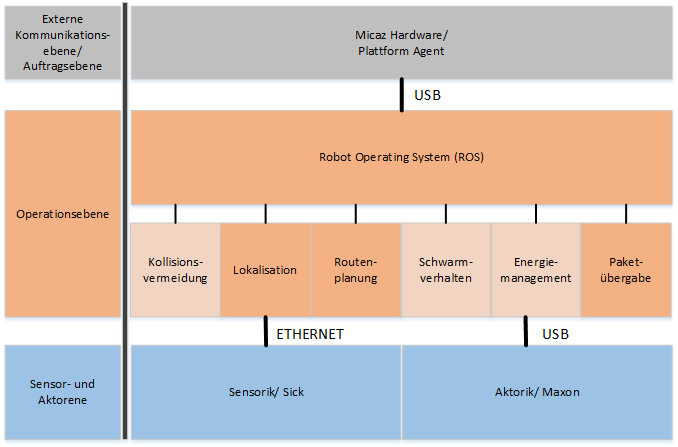
\includegraphics[width=1\textwidth]{DRIVE_Architektur.png}
	\caption{Architektur des Volksbot}
	\label{fig:architecture_volksbot}
\end{figure}

Die in dunkleren rot hervorgehobenen Funktionen der Operationsebene deuten deren höhere Wichtigkeit an und geben ein erstes Anzeichen darauf welche Funktionen erfolgreich umgesetzt werden konnten.

\subsection{Implementierung}
Einführung in den Quellcode
\begin{itemize}
\item Was machen die Dateien? 
\item Diagramm Michael

werden im Moment überarbeitet

\end{itemize}
Wegfindung/ Navigation
\begin{itemize}
\item Odemetrie, Laserscan
\end{itemize}
Hub, Flow
Kommunikation Volksbot, Micaz, Materialfluss

\subsection{Erreichte Funktionalitäten}

\textbf{Beschreibung eines Szenarios mit dem bisher implementierten Volksbot}:

Mit Hilfe des Sick LMS100 Laserscanners wurde eine statische Umgebungskarte generiert, welche den Volksbots bekannt ist. Innerhalb dieser Karte hat ein Volksbot einen zuvor definierten Startpunkt den er für seine eigene Lokalisierung benötigt. Mit Hilfe des MICAZ Moduls kann der Volksbot Aufträge von den Rampen annehmen und beginnt mit der Abarbeitung, indem er mit dem DijkStra Suchalgorithmus die Route bestimmt.Während der Fahrt arbeitet der Volksbot mit Odometrie und dem Laserscanner um seine aktuelle Position zu bestimmen und seine Route aktuell zu halten, ausserdem passt er die Höhe seines Hubs dem Auftrag an. Das bedeutet das er ensprechend seiner Auftragsart den Hub hoch oder runter fährt, damit er das Paket annehmnen oder abgeben kann. Sobald der Volksbot die Zielrampe erreicht hat , richtet er seine Position aus und nähert sich mit einem gewissen Sicherheitsabstand der Rampe. Zur Annahme oder Abgabe des Paketes wird das Förderband in Bewegung gesetzt und läuft solange, bis die Sensoren, welche sich an dem Förderband befinden, das Paket vollständig auf dem Förderband lokalisiert haben oder sich bei der Abgabe kein Paket mehr auf dem Förderband befindet. Sollte der Volksbot ein Paket erhalten haben, so berechnet er die neue Route zum Ziel und fährt diese ab, ansonten wartet er auf den nächsten Auftrag.

\subsection{Herausforderungen}

Bei der Implementierung der Funktionen des Volksbot traten einige Herausforderungen auf, deren Lösungen besonderen Aufwand hervorriefen oder nicht umgesetzt wurden. Ein Beispiel dafür ist die Selbstlokalisation des Roboters durch die Odometrieberechnung und dessen Verbesserung durch die adaptive Monte Carlo Lokalisation (AMCL). Aufgrund der Fehleranfälligkeit der einfachen Odometrie durch Einflüsse wie die Beschaffenheit des Bodens oder Unterschiede im Reifendruck, ist der Einsatz von Algorithmen wie die adaptive Monte Carlo Lokalisation, welcher die Daten des Laserscanners nutzt, notwendig.  Die Qualität der Odometrie musste durch das Kalibrieren des Parameters der Achsenlänge des Roboters erhöht werden, um die nötige Voraussetzung für einen funktionierenden AMCL-Algorithmus zu schaffen. Eine gute Odometrie lässt sich dadurch erkennen, dass die Punkte des Laserscans auch bei Bewegung weiterhin mit den Wänden der Umgebungskarte übereinstimmen. Durch die Verwendung der Selbstlokalisation über AMCL führt der Roboter während seiner Navigation Drehungen um die eigene Achse aus, um seine Position zu berechnen. Dieses Verhalten führt dazu, dass der Roboter deutlich mehr Zeit als vermutet benötigt, um seinen Weg zurückzulegen. Bei der Parametrisierung für die Wegplanung und des AMCL-Algorithmus musste ein Gleichgewicht zwischen Schnelligkeit und Genauigkeit gefunden werden, um ein stabiles System zu schaffen. Durch die Vielzahl der Möglichkeiten war die Suche nach geeigneten Einstellungen problematisch.  

Eine weitere Herausforderung stellt die Erkennung von Hindernissen dar, die ober- oder unterhalb des Laserscanners in den Raum ragen. Zur Lösung dieses Problems könnte ein weiterer bildgebender Sensor genutzt werden, um den gesamten Raum nach potenziellen Hindernissen zu untersuchen.

Mit großem Aufwand war die korrekte Ansteuerung der Maxon Controller verbunden. Besonders die Parametrisierung des kleineren Maxon Controllers unter ROS, welcher für den Betrieb des Förderbandes verwendet wird, stellte sich als Problem heraus. Schon kleinere Abweichungen der Parameter für Spannungs- und Beschleunigungswerte in der Ansteuerung des Controllers führten zu Systemabstürzen.
 
Die Programmierung und Parametrisierung der Teilfunktionen musste mit Blick auf
die CPU-Auslastung der Steuereinheit geschehen, da einige Berechnungen bei falscher
Verwendung zu sehr hohen Auslastungen und einer unzureichenden Performance des
Roboters führten.



\subsection{Ausblick}

Der Volksbot sollte um folgende Funktionalitäten erweitert werden:

\begin{itemize}

\item \textbf{Genauigkeit bei der Übergabe}: Die Genauigkeit des Heranfahrens an eine Zielposition, wie z.B. den Ausgang einer Rampe, muss verbessert werden, um eine erfolgreiche Übergabe zu gewährleisten. Der Volksbot stürzt bei direktem anfahren an die Rampe ab, da der Bewegungsraum eingeschränkt wird.

\item \textbf{Kollisionserkennung mobile Hindernisse - Schwarmverhalten}: Der Volksbot sollte Hindernisse, die sich selbstständig bewegen, erkennen und entsprechend reagieren. Dies könnte beim erkennen eines Objektes mittels einer Neuplanung der Route, einer kurzen Unterbrechung der Fahrt oder eines Ausweichmanövers umgesetzt werden.

\item \textbf{Rückkopplung an Simulation}: Die Volksbots sollten ihre aktuelle Position, sowie den Beladungs- und Eneriezustand an die Simulation zurückgeben.

\item \textbf{Fahralgorithmus}: Es können alternative Alorithmen implementiert werden, um die Berechnungszeiten zu verkürzen oder optimalere Routen zu finden.

\item \textbf{Kostenabschätzung}: Eine optimale Berechnung zur Bestiimmung der benötigten Zeit, Strecke und Energieverbrauchs würde die Jobverteilung effizienter gestalten.

\item \textbf{Ladestation}: Die Ladestation muss angebracht und getestet werde. Danach fehlt die automatische Erkennung des kritischen Zustandes, sowie das selbstständige anfahren der Ladestation, damit der Akku geladen werden kann. Hierbei handelt es sich um einen Prototypen der noch getestet werden muss.

\end{itemize}



